% !TEX root = ../main.tex
% 本文件由 build-tex.sh 从 23-DSP指南-第23章中译.md 生成，改内容请改 md 后重新生成

\chapter{图像的形成与显示}\label{ch-23}

图像描述的是某个参数在一个面上如何变化。例如，普通的可见光图像来自光强在二维平面上的变化。不过，科学成像用的参数并不只有光。例如，图像可以由集成电路的温度、病人动脉中的血流速度、遥远星系发出的
X
射线、地震时的地面运动等构成。这些特殊的图像通常会被转换成普通的图片（即光学图像），以便用人眼来判读。作为图像处理的第一章，本章介绍数字图像是怎样形成、又是怎样呈现给观察者的。

\section{数字图像的结构}

图 23-1
展示了数字图像的结构。这幅示例图像是金星，由环绕它飞行的空间探测器用微波雷达拍摄。之所以要用微波成像，是因为金星浓密的大气挡住了可见光，普通照相根本行不通。图中的图像由
40,000 个采样组成，排成 200 列 × 200
行的二维数组。和一维信号一样，这些行和列可以编号为 0 到
199，也可以编号为 1 到
200。按图像处理的行话，每个采样叫做一个像素(pixel)，是 picture
element（图像元素）的缩写。本例中每个像素是一个 0 到 255
之间的数。拍摄时，这个数对应行星表面相应位置反射回来的微波能量的多少。为了把它显示成可见的图像，每个像素的值被转换成一个灰度(grayscale)：0
是黑，255 是白，中间的值是深浅不同的灰。

\begin{figure}[htbp]
\centering
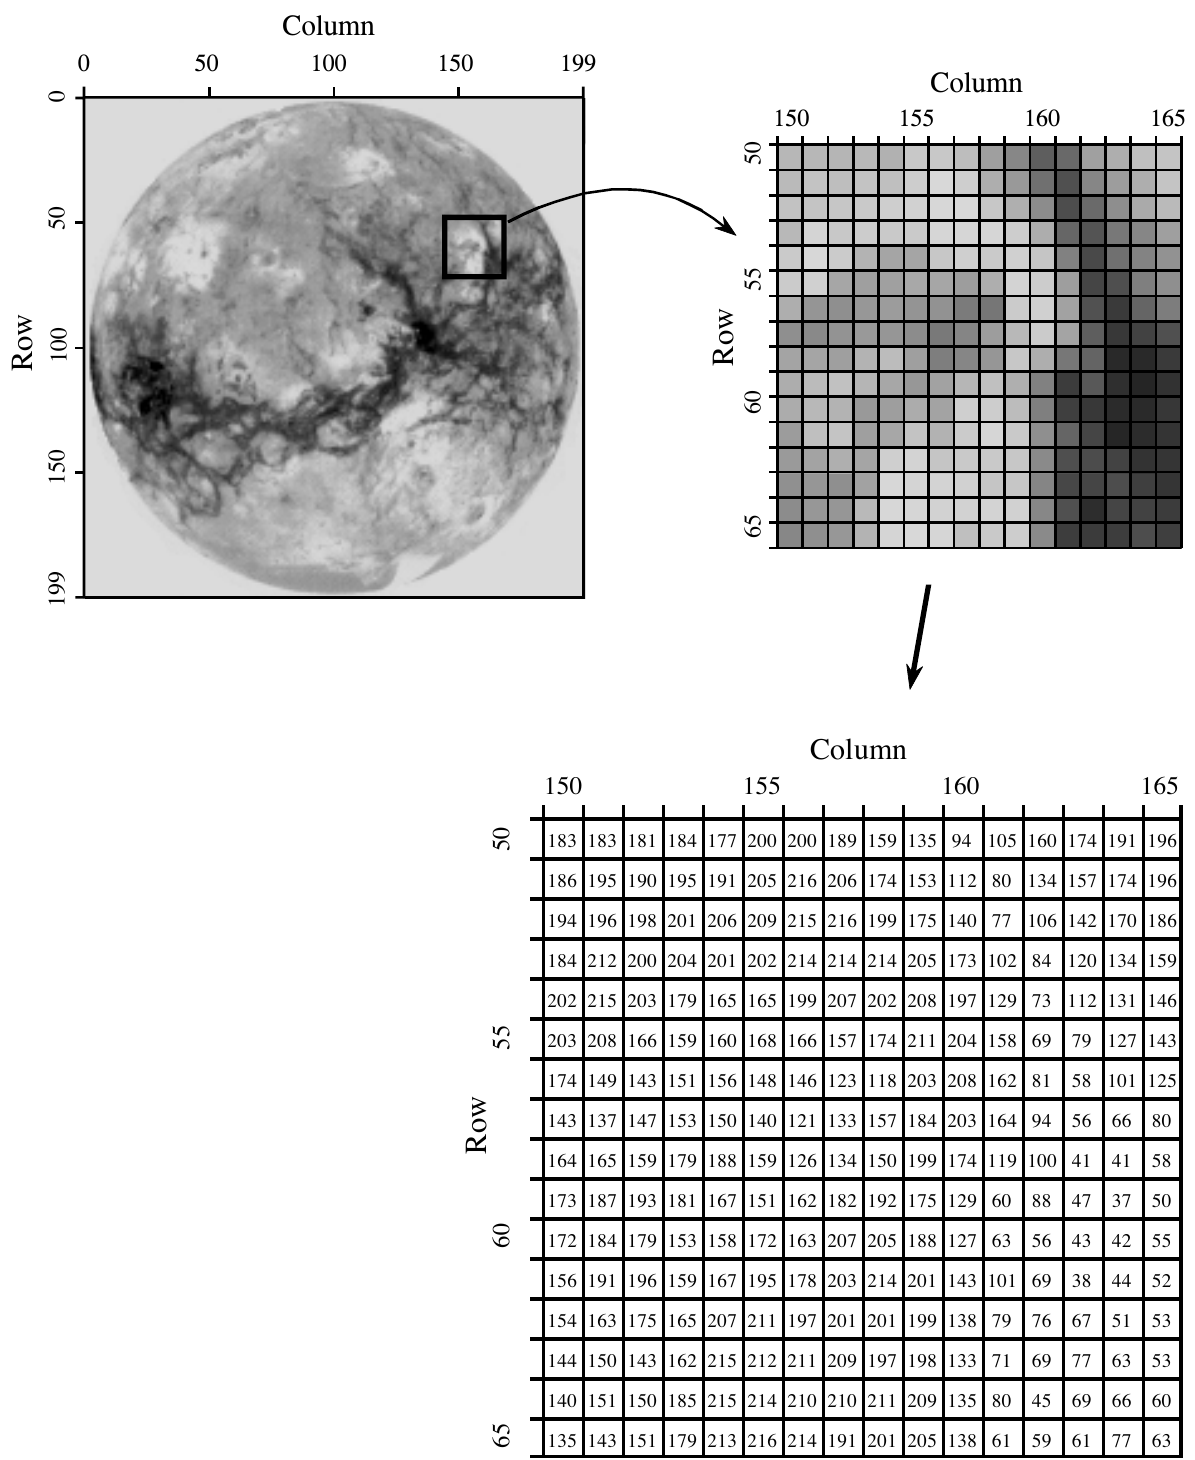
\includegraphics[width=0.996\linewidth,height=0.8\textheight,keepaspectratio]{assets/ch23/fig23-01.png}
\caption*{\textbf{图 23-1　数字图像的结构。}
这幅示例图像是以反射微波观察到的金星。数字图像用一个二维数组表示，数组里的每个数叫做一个像素。本图中数组为
200 行 × 200 列，每个像素是 0 到 255
之间的一个数。拍摄时，每个像素的值对应反射回来的微波能量的强弱。把
0～255 的每个值对应到深浅不同的灰色，就形成了灰度图像。 （Column =
列，Row = 行。左上是整幅图，右上是方框区域（第 50～65 行、第 150～165
列）放大后的像素格，下方是这些像素的数值。原书图注排在图左下，裁图时已去掉，译文见上。）}
\end{figure}

图像的信息编码在空间域(spatial
domain)中，空间域相当于图像版的时域。换句话说，图像中的特征是用边缘(edge)来表示的，而不是用正弦波。这意味着像素的间距和数量，取决于需要看清多小的特征，而不是取决于采样定理的形式约束。图像中也会出现混叠(aliasing)，但它一般被看作一种小麻烦，而不是大问题。例如，细条纹西装在电视上看起来很糟糕，因为这种重复图案的频率超过了奈奎斯特频率(Nyquist
frequency)。混叠出来的频率表现为明暗相间的条带，随着人的走动在衣服上移动。

一幅''典型''的数字图像大约由 500 行 × 500
列组成。这是电视、个人计算机应用和一般科研中常见的图像质量。像素更少的图像，比如
250 ×
250，被认为分辨率异常低。新出现的成像方式往往就是这样；随着技术成熟，像素会越来越多。这种低分辨率图像看起来明显不自然，常常能看到一个个像素。另一端，超过
1000 × 1000 像素的图像被认为质量特别好，这是最好的计算机图形、高清电视和
35
毫米电影的质量。还有一些应用需要更高的分辨率，每边几千个像素：数字化的 X
光片、太空照片，以及杂志上的光面广告。

使用较低分辨率图像最大的动力在于要处理的像素更少。这不是小事；图像处理中最难的问题之一，就是管理海量的数据。例如，一秒钟的数字音频大约需要
8 千字节，而一秒钟的电视大约需要 8 兆字节。用 33.6 kbps
的调制解调器传送一幅 500 × 500 像素的图像，要将近一分钟！图像尺寸跳到
1000 × 1000，这些问题就翻两番。

\begin{quote}
\textbf{译注：} ``一秒钟数字音频约 8 千字节''对应的是电话质量（8 kHz
采样、每采样 8 位）；CD 音质（44.1 kHz、16 位、立体声）约为每秒 176
千字节。
\end{quote}

图像处理中通常用 256
个灰度级（量化级），对应每像素一个字节。这样做有几个原因。第一，单个字节便于数据管理，因为计算机通常就是这样存储数据的。第二，图像中像素数量巨大，这在一定程度上弥补了量化级数的不足。例如，设想一组相邻像素的值在数字编号（digital
number，DN）145 和 146 之间交替。人眼会把这片区域感知为亮度
145.5。换句话说，图像本身带有很强的抖动(dithering)效果。第三，也是最重要的一点：1/256（0.39\%）的亮度步长，比人眼能察觉的还小。呈现给人看的图像，用超过
256 级也不会变得更好。

不过，有些图像需要以每像素超过 8 位的精度来存储。记住，DSP
中遇到的大多数图像表示的是非视觉参数。采集到的图像可能需要更多的量化级，才能恰当地捕捉信号的细微之处。重点在于：不要指望人眼能看出这些细密的级别中包含的全部信息。后面讨论亮度和对比度时，我们会考虑怎样绕开这个问题。

数字图像中每个像素的值，代表被数字化的连续图像中的一小块区域。例如，设想金星探测器在环绕飞行时，沿行星表面每隔
10 米取一个样。这就定义了一个方形的采样间距和采样网格(sampling
grid)，每个像素代表一块 10 米 × 10
米的区域。现在设想一次微波反射测量中发生了什么。探测器发出一束高度聚焦的微波能量，照到地面上的，比如说，是一块直径
15
米的圆形区域。因此，不管采样网格多大，每个像素所含的都是这块圆形区域的信息。

连续图像中对像素值有贡献的这块区域，叫做采样孔径(sampling
aperture)。采样孔径的大小通常与所用成像系统的固有能力有关。例如，显微镜受光学元件质量和光波长的限制，电子相机受图像传感器中电子随机扩散的限制，等等。大多数情况下，采样网格做得与系统的采样孔径大致相同。最终数字图像的分辨率，主要受这两者中较大的那个限制：采样网格或采样孔径。第
25 章讨论数字图像的空间分辨率时，我们会回到这个话题。

给数字图像加上颜色的办法，是每个像素用三个数，分别表示三种原色------红、绿、蓝------的强度。混合这三种颜色可以产生人眼能感知的所有颜色。每种颜色的强度通常用一个字节存储，于是图像总共能表示
256×256×256 = 1680 万种不同的颜色。

当目的是向观众呈现世界的真实画面时，比如电视和照片，颜色非常重要。但科学和工程中的图像通常不是这样用的。这里的目的是把人的视觉系统当作工具，去分析一个二维信号。黑白图像就足够了。

\section{相机与眼睛}

眼睛的结构和工作方式与电子相机非常相似，放在一起讨论很自然。两者都基于两个主要部件：镜头组件和成像传感器(imaging
sensor)。镜头组件收集物体发出的一部分光，把它聚焦到成像传感器上。成像传感器再把光的图案转换成视频信号，可能是电信号，也可能是神经信号。

图 23-2
展示了透镜的工作方式。在这个例子中，一位滑冰者的像被聚焦到一块屏幕上。聚焦(focus)的意思是：滑冰者身上的每一点，都与屏幕上的一个对应点一一对应。例如，考虑脚尖上
1 mm × 1 mm 的一块区域。在明亮的光线下，每秒大约有 100
万亿个光子打到这一平方毫米上。根据表面性质的不同，这些入射光子中有 1\%
到 99\%
会被反射到随机的方向。被反射的光子中只有很小一部分会穿过透镜。例如，一个距离物体
3 米、直径 1 厘米的透镜，只能接收到大约百万分之一的反射光。

\begin{figure}[htbp]
\centering
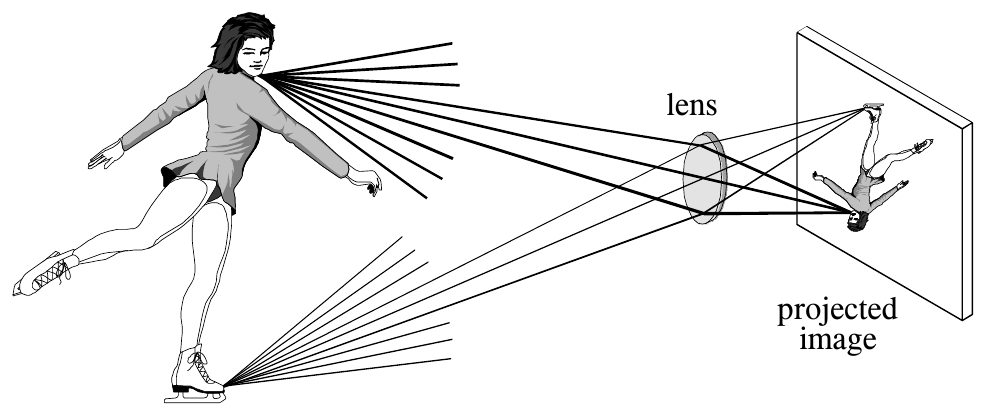
\includegraphics[width=0.821\linewidth,height=0.8\textheight,keepaspectratio]{assets/ch23/fig23-02.png}
\caption*{\textbf{图 23-2　透镜的聚焦。}
透镜收集从一个点光源发散出来的光，迫使它们在另一个位置重新会聚成一个点。这使得透镜能把像投射到一个面上。
（lens = 透镜，projected image = 投射的像。）}
\end{figure}

透镜中的折射(refraction)会改变每个光子的方向，改变多少取决于光子打到玻璃/空气界面的位置和角度。这些方向变化使得从一个点发散出去的光，在投影屏上重新会聚到一个点。从脚尖反射并穿过透镜的所有光子，都在投射的像中的''脚尖''处重新汇合。同理，物体上任何一点发出的光，都有一部分会穿过透镜，并聚焦到投射的像中的对应点。

图 23-3 和图 23-4
分别画出了电子相机和人眼的主要结构。两者都是不透光的外壳，一端装着透镜，另一端是图像传感器。相机里充满空气，而眼睛里充满透明液体。每个透镜系统都有两个可调参数：焦距和光圈(iris)直径。

\begin{figure}[htbp]
\centering
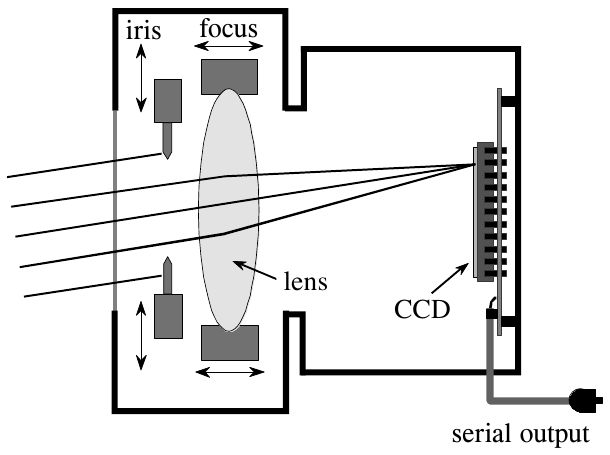
\includegraphics[width=0.508\linewidth,height=0.8\textheight,keepaspectratio]{assets/ch23/fig23-03.png}
\caption*{\textbf{图 23-3　电子相机示意图。}
聚焦是通过让镜头靠近或远离成像传感器来实现的。到达传感器的光量由光圈控制，光圈是一个改变镜头有效直径的机械装置。当今相机中最常见的成像传感器是
CCD，即一个由感光元件组成的二维阵列。 （iris = 光圈，focus = 调焦，lens
= 镜头，CCD = 电荷耦合器件，serial output =
串行输出。原书图注排在图左侧，裁图时已去掉，译文见上。）}
\end{figure}

\begin{figure}[htbp]
\centering
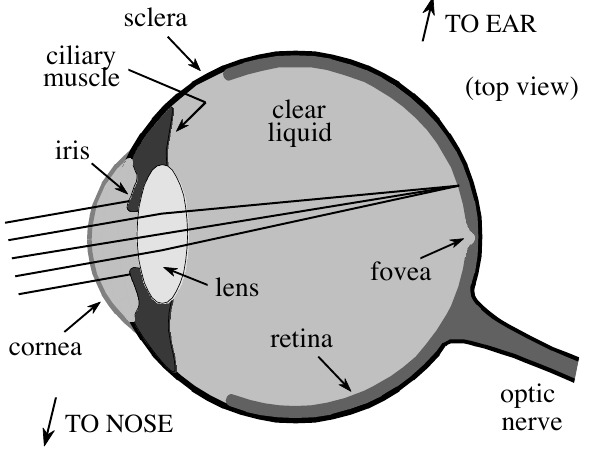
\includegraphics[width=0.492\linewidth,height=0.8\textheight,keepaspectratio]{assets/ch23/fig23-04.png}
\caption*{\textbf{图 23-4　人眼示意图。} 眼睛是一个充满液体、直径约 3
厘米的球体，外面包着一层坚韧的外壳，叫巩膜。聚焦主要由角膜完成，角膜是眼睛前部一个固定的透镜。焦距的调节靠收缩连在眼内柔性晶状体上的肌肉来实现。进入眼睛的光量由虹膜控制，虹膜由不透明的肌肉组织构成，遮住晶状体的一部分。眼球的后半球是视网膜，这是一层感光神经细胞，把像转换成视神经中的神经信号。
（sclera = 巩膜，ciliary muscle = 睫状肌，iris = 虹膜，clear liquid =
透明液体，lens = 晶状体，cornea = 角膜，fovea = 中央凹，retina =
视网膜，optic nerve = 视神经，TO EAR = 朝耳朵，TO NOSE = 朝鼻子，top
view = 俯视图。原书图注排在图左侧，裁图时已去掉，译文见上。）}
\end{figure}

如果透镜没有正确聚焦，物体上的每一点都会投射到成像传感器上的一个圆形区域，使像变模糊。在相机中，聚焦是靠物理地移动镜头、使它靠近或远离成像传感器来实现的。相比之下，眼睛里有两个透镜：眼球前部的一个凸起，叫角膜(cornea)；以及眼内一个可调的透镜，即晶状体。光的折射大部分由角膜完成，但角膜的形状和位置是固定的。焦距的调节由内部的晶状体完成，它是一种柔性结构，可以在睫状肌(ciliary
muscle)的作用下变形。这些肌肉收缩时，晶状体变扁，使物体清晰成像。

\begin{quote}
\textbf{译注：}
原书此处说''肌肉收缩时晶状体变扁''。按目前生理学的通常解释，睫状肌收缩时悬韧带放松，晶状体变得更凸（用于看近处）；睫状肌放松时晶状体被拉扁（用于看远处）。译文照原书翻译，供参考。
\end{quote}

在两种系统中，光圈都用来控制透镜有多少面积暴露在光下，从而控制投射到成像传感器上的像的亮度。眼睛的虹膜(iris)由不透明的肌肉组织构成，收缩时会使瞳孔(pupil，即透光的开口)变大。相机的光圈则是完成同样功能的机械组件。

光学系统中的各个参数会以许多意想不到的方式相互影响。例如，考虑可用光量和光传感器的灵敏度怎样影响所得图像的清晰度。之所以有影响，是因为光圈直径和曝光时间要调节到恰好把适量的光从景物传到图像传感器上。如果光线充足，就可以缩小光圈直径，从而得到更大的景深(depth-of-field，即物体保持清晰的那段距相机的距离范围)。当物体处于不同距离时，更大的景深能给出更清晰的图像。此外，光线充足还能缩短曝光时间，减少相机抖动和物体运动造成的模糊。光学系统中充满了这类取舍。

相机和眼睛都需要可调的光圈，因为环境中光强的范围远大于光传感器能直接处理的范围。例如，阳光和月光的光强相差大约一百万倍。再加上反射率可以在
1\% 到 99\% 之间变化，光强的范围就接近一亿倍。

电子相机的动态范围(dynamic range)通常是 300 到
1000，定义为器件能测量的最大信号除以器件的固有噪声。换句话说，产生的最大信号是
1 伏，而在黑暗中的均方根噪声约为 1
毫伏。典型的相机镜头，光圈能把通光面积改变约 300
倍。这使得典型电子相机的动态范围达到几十万。显然，在明亮阳光下用的相机和镜头组件，到了漆黑的夜里就没法用了。

相比之下，眼睛的动态范围几乎覆盖了环境中的巨大变化。出人意料的是，实现这一巨大动态范围的主要手段并不是虹膜。从暗到亮，瞳孔的面积只变化约
20
倍。剩下的动态范围，靠感光神经细胞逐渐调整自身的灵敏度来应付。例如，走进漆黑的电影院后，眼睛要花几分钟才能适应弱光。

DSP
改善图像的一种方法，是减小观察者需要面对的动态范围。也就是说，我们不希望同一幅图像中既有很亮的区域又有很暗的区域。一幅反射图像由两个图像信号构成：景物被照明的二维分布，乘以景物反射率的二维分布。反射率分布的动态范围小于
100，因为所有普通材料都反射入射光的 1\% 到
99\%。图像的大部分信息都包含在这里，比如物体在景物中的位置以及它们的表面特征。相比之下，照明信号取决于物体周围的光源，而不取决于物体本身。照明信号的动态范围可以达到几百万，不过在单幅图像中更典型的是
10 到
100。照明信号携带的有用信息很少，却会因为增大动态范围而使最终图像变差。DSP
可以通过抑制照明信号、让反射率信号在图像中占主导来改善这种情况。下一章会介绍实现这一算法的一种方法。

覆盖在眼球后部的感光表面叫视网膜(retina)。如图 23-5
所示，视网膜可以分成三层主要的特化神经细胞：一层把光转换成神经信号，一层做图像处理，一层把信息传给通向大脑的视神经(optic
nerve)。在几乎所有动物中，这些层的排列方向看起来都是反的。也就是说，感光细胞在最后一层，光要先穿过其他层才能被检测到。

\begin{figure}[htbp]
\centering
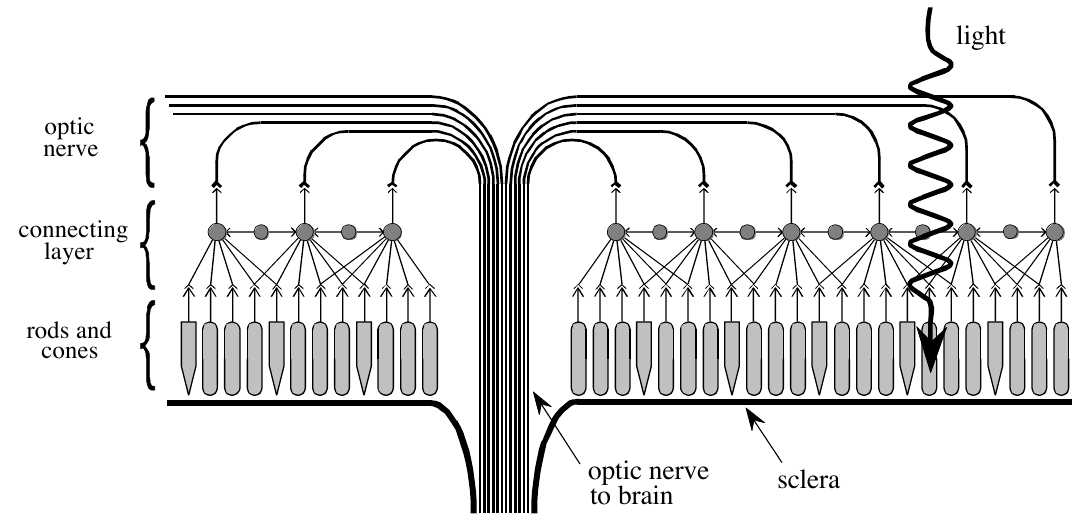
\includegraphics[width=0.908\linewidth,height=0.8\textheight,keepaspectratio]{assets/ch23/fig23-05.png}
\caption*{\textbf{图 23-5　人的视网膜。} 视网膜包含三个主要层次：(1)
视杆细胞和视锥细胞这两种感光器；(2) 中间层，负责数据压缩和图像处理；(3)
通向大脑的视神经纤维。这几层的结构看起来是反的，光要先穿过其他层才能到达感光器。
（optic nerve = 视神经，connecting layer = 连接层，rods and cones =
视杆细胞和视锥细胞，light = 光，optic nerve to brain =
通向大脑的视神经，sclera = 巩膜。原书图注中的 principle 应为
principal。）}
\end{figure}

检测光的细胞有两种：视杆细胞(rod)和视锥细胞(cone)，名字来自它们在显微镜下的外形。视杆细胞专门在光线很弱时工作，比如在夜空下。在接近全黑的环境中，视觉显得噪声很大，也就是说，像里布满了不断变化的颗粒状图案。这是因为图像信号非常弱，而不是眼睛本身的缺陷。进入眼睛的光太少了，以至于能看到单个光子的随机检测。这叫统计噪声(statistical
noise)，所有弱光成像中都会遇到，比如军用夜视系统。第 25
章会再讲这个话题。由于视杆细胞不能分辨颜色，弱光下的视觉是黑白的。

视锥细胞专门用来分辨颜色，但只有在光线较充足时才能工作。眼睛里有三种视锥细胞：对红光敏感的、对绿光敏感的和对蓝光敏感的。这是因为它们含有不同的感光色素(photopigment)，即吸收不同波长（颜色）光的化学物质。图
23-6 给出了能触发这三种感光器的光的波长。这叫 RGB
编码，颜色信息就是以这种形式通过视神经离开眼睛的。由于大脑低层的神经处理，人对颜色的感知变得更加复杂。RGB
编码被转换成另一种编码方案，把颜色分为：红或绿、蓝或黄、亮或暗。

\begin{figure}[htbp]
\centering
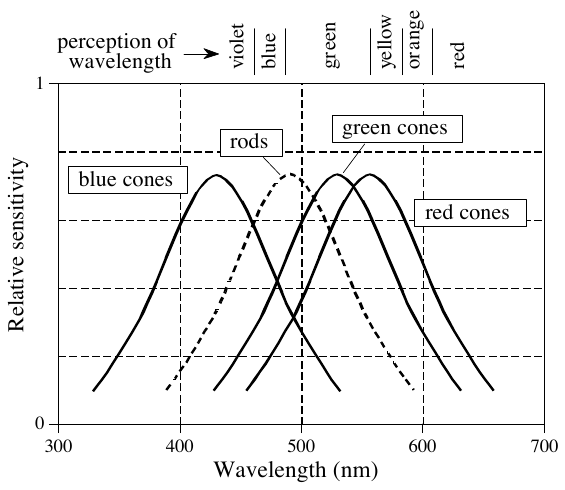
\includegraphics[width=0.471\linewidth,height=0.8\textheight,keepaspectratio]{assets/ch23/fig23-06.png}
\caption*{\textbf{图 23-6　眼睛的光谱响应。}
人眼中的三种视锥细胞分别对光谱的不同部分有响应，大致对应红、绿、蓝。这三者的组合构成了人能感知的所有颜色。视锥细胞的灵敏度不够，无法在弱光环境中工作，这时由视杆细胞来检测图像。这就是夜里难以分辨颜色的原因。
（Relative sensitivity = 相对灵敏度，Wavelength (nm) =
波长（纳米）；blue cones = 蓝视锥细胞，rods = 视杆细胞，green cones =
绿视锥细胞，red cones = 红视锥细胞；perception of wavelength =
对波长的感知：violet 紫、blue 蓝、green 绿、yellow 黄、orange 橙、red
红。原书图注排在图左侧，裁图时已去掉，译文见上。）}
\end{figure}

RGB
编码是人类视觉的一个重要局限：环境中存在的各种波长，被笼统地归入仅仅三大类。相比之下，专用相机能把光谱分成数百乃至数千种不同的颜色。例如，可以用它们把细胞分类为癌变或健康、了解遥远恒星的物理性质，或者发现藏在森林里的伪装士兵。为什么眼睛在分辨颜色方面如此有限？显然，人类生存所需的，只是在绿叶之间、蓝天背景下找到一个红苹果。

视杆细胞和视锥细胞大约 3 μm 宽，紧密地排满视网膜整个 3 cm × 3 cm
的表面。于是视网膜由大约 10,000 × 10,000 = 1
亿个感光器组成的阵列构成。相比之下，视神经只有大约一百万根神经纤维与这些细胞相连。平均来说，每根视神经纤维通过连接层与大约
100
个感光器相连。除了汇总信息，连接层还会增强图像：锐化边缘，并抑制景物中的照明成分。这种生物图像处理将在下一章讨论。

视网膜正中央有一小块区域，叫中央凹(fovea，拉丁语''凹坑''的意思)，用于高分辨率视觉（见图
23-4）。中央凹在几个方面与视网膜其他部分不同。第一，视神经和连接层被推到中央凹的两侧，让感光器更直接地暴露在入射光下。这使得中央凹看起来是视网膜上的一个小凹陷。第二，中央凹里只有视锥细胞，而且排列得比视网膜其他部分更紧密。中央凹里没有视杆细胞，这解释了为什么夜里看东西时，眼睛稍微偏向物体一侧往往比直视看得更清楚。第三，每根视神经纤维只受少数几个视锥细胞影响，因而定位能力很好。中央凹小得出奇。在正常阅读距离上，中央凹只能看到直径约
1 毫米的区域，比一个字母还小！这块区域内的分辨率大约相当于 20×20
的像素网格。

人的视觉靠一种叫扫视(saccade)的跳跃式眼动来弥补中央凹太小的缺陷。这些突然的运动让高分辨率的中央凹能快速扫过视野，寻找相关信息。此外，扫视使视杆细胞和视锥细胞面对的光图案不断变化。这一点很重要，因为视网膜天然会适应光强的变化。事实上，如果强迫眼睛一直盯着同一个景物不动，几秒钟后细节和颜色就开始消退。

电子相机中最常用的图像传感器是电荷耦合器件(charge coupled
device，CCD)。CCD 是一种集成电路，在 1980
年代取代了大部分真空管摄像机，就像二十年前晶体管取代了真空管放大器一样。CCD
的核心是一片薄薄的硅片，通常约 1 平方厘米。如图 23-7
的剖面图所示，背面镀有一层接地的薄金属。正面覆盖着一层很薄的电绝缘层，以及一组重复排列的电极。最常见的
CCD 是三相读出(three phase
readout)型，每隔两个电极连在一起（即每三个一组）。所用的硅叫 p
型硅，意思是它含有过量的正电荷载流子，叫空穴(hole)。在这里的讨论中，可以把空穴想成一个能在硅中自由移动的带正电的粒子。图中空穴用''+``号表示。

\begin{figure}[htbp]
\centering
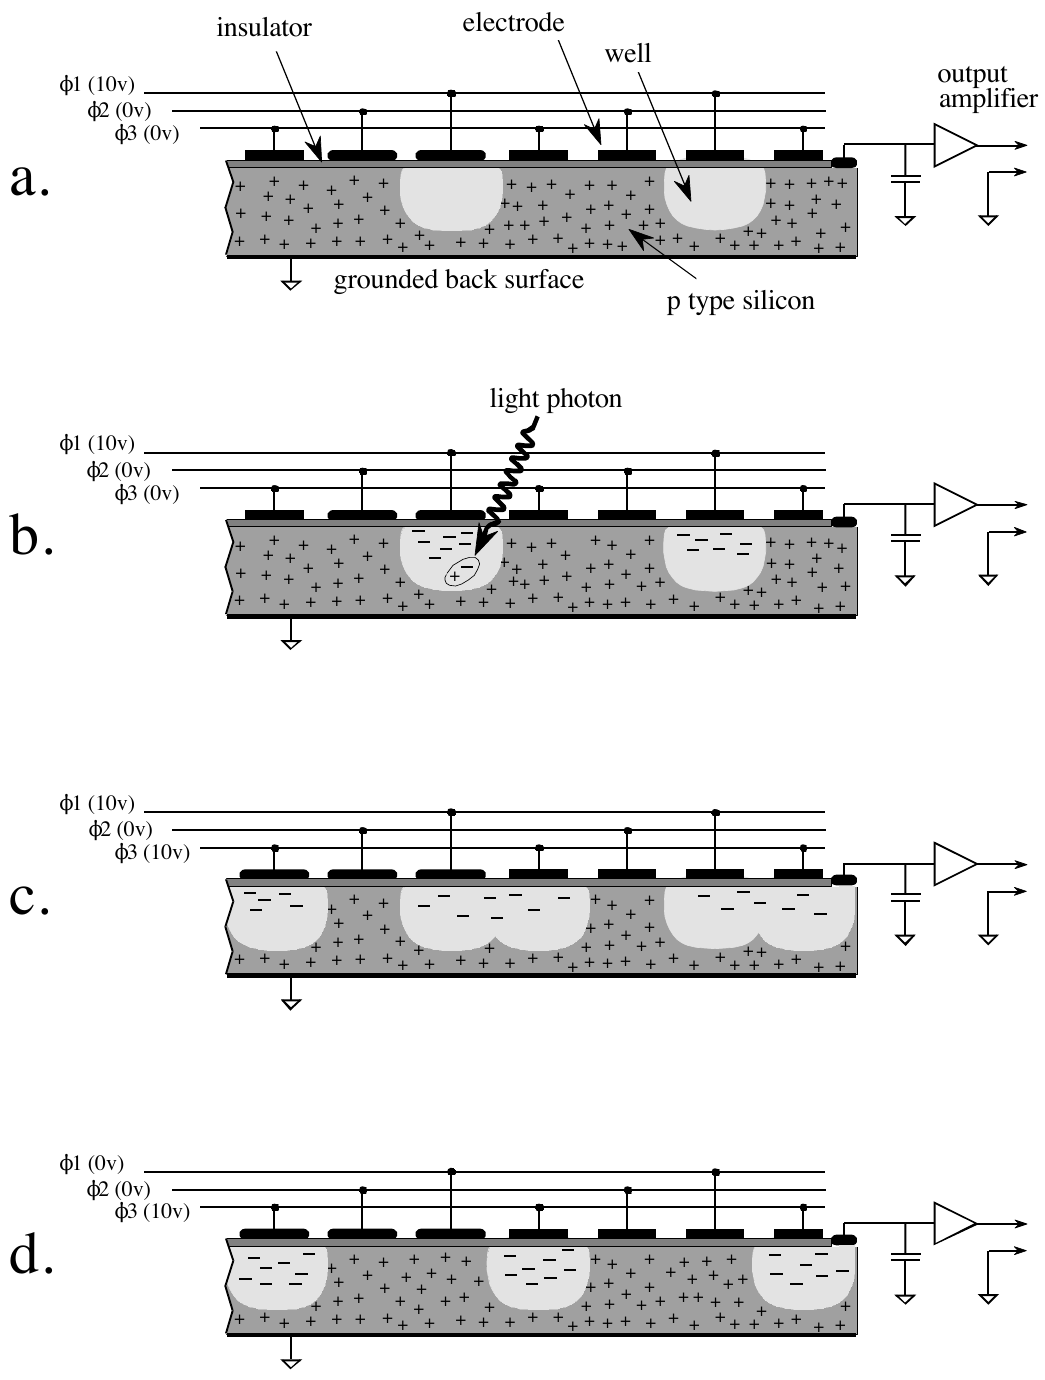
\includegraphics[width=0.871\linewidth,height=0.8\textheight,keepaspectratio]{assets/ch23/fig23-07.png}
\caption*{\textbf{图 23-7　电荷耦合器件（CCD）的工作原理。} 如剖面图所示，一薄片 p
型硅上覆盖着一层绝缘层和一组电极。电极每三个连成一组，可以施加三路独立的电压：φ1、φ2
和
φ3。给某个电极加正电压时，空穴（即用''+``表示的正电荷载流子）被推开，形成一个缺少空穴的区域，叫势阱。入射光产生空穴和电子，使电子在每个势阱中积累起来（用''−``表示）。通过操纵三路电极电压，每个势阱中的电子可以被移到硅片边缘，在那里由一个电荷敏感放大器把电荷转换成电压。
（insulator = 绝缘层，electrode = 电极，well = 势阱，output amplifier =
输出放大器，grounded back surface = 接地的背面，p type silicon = p
型硅，light photon = 光子；φ1 (10v) 等表示各相电极上的电压。）}
\end{figure}

在 (a) 中，三相之一加上 +10 伏电压，另外两相保持 0
伏。这使得空穴从每隔两个的电极下方移开，因为正电荷会被正电压排斥。这就在这些电极下方形成了一个叫阱(well)的区域，是物理术语势阱(potential
well)的简称。

CCD 中的每个阱都是非常高效的光传感器。如 (b)
所示，一个光子打到硅上，它的能量转化为两个带电粒子：一个电子和一个空穴。空穴移走，留下电子困在阱里，被电极上的正电压束缚住。图中电子用''−``号表示。在积分期(integration
period)内，照到 CCD 上的光图案被转换成 CCD
各个阱中的电荷图案。光源越暗，需要的积分期越长。例如，标准电视的积分期是
1/60 秒，而天文摄影可以积累光好几个小时。

电子图像的读出方式相当巧妙：每个阱中积累的电子被推向输出放大器。如 (c)
所示，在两相电极线上加正电压，使每个阱都向右扩展。如 (d)
所示，下一步撤掉第一相的电压，原来的阱随之消失。这样，积累的电子就停留在比起始位置右移一格的阱中。在三相电极线之间重复这种脉冲序列，积累的电子就被一路推向右边，直到到达一个电荷敏感放大器(charge
sensitive
amplifier)。这是''一个电容后面接一个单位增益缓冲器''的花哨名字。电子从最后一个阱被推出时，流到电容上并产生一个电压。为了获得高灵敏度，电容做得极小，通常小于
1 pF。这个电容和放大器是 CCD 的组成部分，做在同一块硅片上。离开 CCD
的信号是一串电压电平，与依次各阱接收到的光量成正比。

图 23-8 展示了怎样从 CCD
读出二维图像。积分期结束后，每个阱中积累的电荷沿着列向上移动，一次移动一行。例如，第
15 行的所有阱先移到第 14 行，再到第 13 行，再到第 12
行，依此类推。每次各行上移时，第 1
行的所有阱都被转移到水平寄存器(horizontal
register)中。水平寄存器是一组特殊的 CCD
阱，能快速地沿水平方向把电荷移到电荷敏感放大器。

\begin{figure}[htbp]
\centering
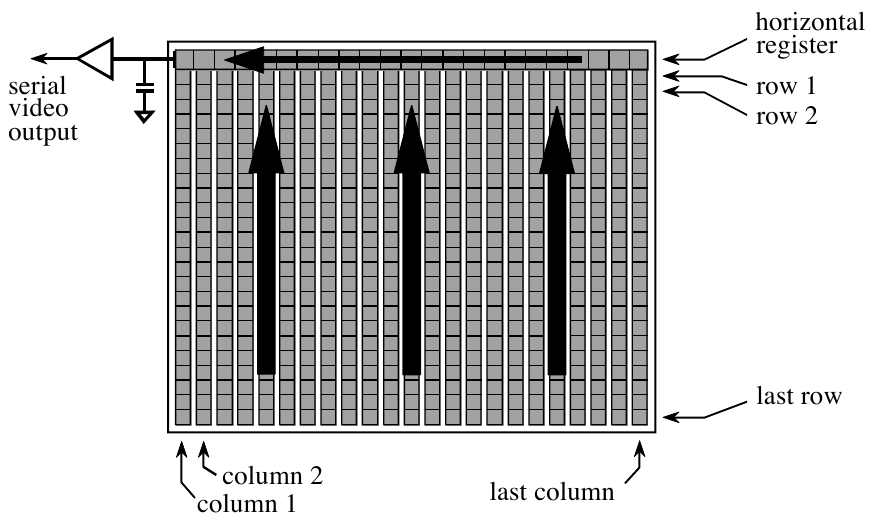
\includegraphics[width=0.729\linewidth,height=0.8\textheight,keepaspectratio]{assets/ch23/fig23-08.png}
\caption*{\textbf{图 23-8　CCD 的结构。} CCD
的成像阱按列排列。读出时，每个阱的电荷沿列向上移入水平寄存器，再由水平寄存器读出到电荷敏感前置放大器。
（serial video output = 串行视频输出，horizontal register =
水平寄存器，row 1 / row 2 = 第 1 行 / 第 2 行，last row =
最后一行，column 1 / column 2 = 第 1 列 / 第 2 列，last column =
最后一列。）}
\end{figure}

注意这种结构把二维数组按一种特定的顺序转换成串行数据流。第一个读出的像素在图像的左上角。然后读出在第一行中从左到右进行，接着在后续各行中也从左到右进行。这叫行优先顺序(row
major order)，把二维数组（图像）转换成顺序数据时几乎总是采用这种顺序。

\section{电视视频信号}

尽管已有 50 多年历史，标准电视信号仍然是传输图像最常用的方式之一。图
23-9 展示了电视信号在示波器上的样子。这叫复合视频(composite
video)，意思是垂直和水平同步(synchronization，sync)脉冲与实际的画面信息混合在一起。电视接收机用这些脉冲来同步垂直和水平偏转电路，使之与正在显示的视频相匹配。标准视频每秒包含
30 幅完整的图像，通常叫帧(frame)。视频工程师会说每帧包含 525
行(line)，这是电视行话，相当于程序员说的''行''(row)。这个数字有点误导，因为其中只有
480 到 486 行包含视频信息；其余 39 到 45
行留给同步脉冲，用来让电视的电路与视频信号保持同步。

标准电视采用隔行扫描(interlaced)格式，以减少显示图像的闪烁。这意味着每帧的所有奇数行先传送，然后再传送偶数行。奇数行的那一组叫奇数场(odd
field)，偶数行的那一组叫偶数场(even
field)。由于每帧由两场组成，视频信号每秒传送 60 场。每一场以一串持续 1.3
毫秒的复杂垂直同步脉冲开始，后面是偶数行或奇数行的视频。每行持续 63.5
微秒，其中包括一个 10.2
微秒的水平同步脉冲，把一行与下一行隔开。在每一行之内，模拟电压对应图像的灰度，越亮的值越远离同步脉冲的方向。这使同步脉冲落在黑色范围之外。按视频行话，同步脉冲被称为''比黑更黑''(blacker
than black)。

\begin{figure}[htbp]
\centering
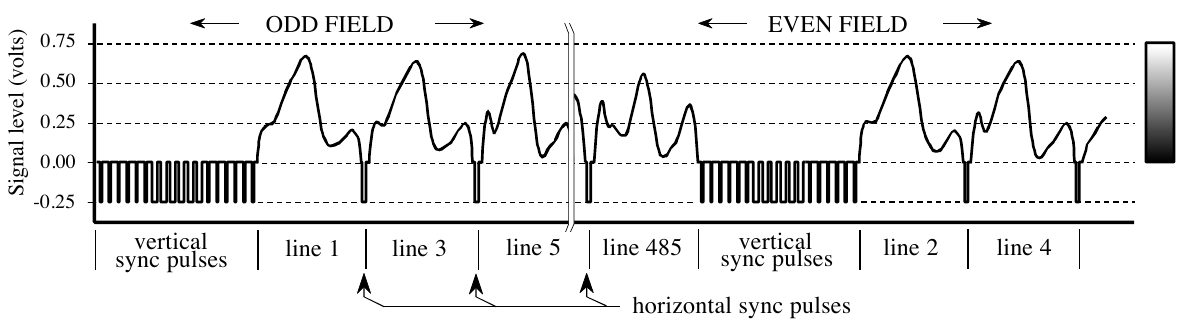
\includegraphics[width=0.988\linewidth,height=0.8\textheight,keepaspectratio]{assets/ch23/fig23-09.png}
\caption*{\textbf{图 23-9　复合视频。} NTSC 视频信号每秒由 30
个完整的帧（图像）组成，每帧包含 480 到 486
行视频。每帧分成两场，一场包含奇数行，另一场包含偶数行。每一场以一组垂直同步脉冲开始，后面是由水平同步脉冲隔开的一行行视频信息。（本图横轴没有按比例绘制。）
（Signal level (volts) = 信号电平（伏），ODD FIELD = 奇数场，EVEN FIELD
= 偶数场，vertical sync pulses = 垂直同步脉冲，horizontal sync pulses =
水平同步脉冲，line 1 / line 3 \ldots{} = 第 1 行 / 第 3 行
\ldots；右侧灰度条表示电平与亮度的对应关系。）}
\end{figure}

用于视频信号模数转换的硬件叫帧采集卡(frame
grabber)。它通常是一块插在计算机里的电子板卡，通过同轴电缆连接相机。收到软件的命令后，帧采集卡等待下一帧开始，即等待垂直同步脉冲。在随后的两场中，每一行视频被采样许多次，通常每行
512、640 或 720 个采样，每个采样 8
位。这些采样作为数字图像的一行存储在内存中。

这种获取数字图像的方式，导致垂直方向和水平方向之间有一个重要的差别。数字图像中的每一行对应视频信号中的一行，因而也对应
CCD 中的一行阱。可惜列就没这么直截了当了。在 CCD 中，每行包含大约 400 到
800 个阱（列），具体取决于所用的器件。从 CCD
读出一行阱时，得到的那行视频被滤波成一个平滑的模拟信号，就像图 23-9
中那样。换句话说，视频信号与 CCD
有多少列无关。水平方向的分辨率受限于模拟信号被允许变化的快慢。彩色电视中这一般设为
3.2 MHz，对应约 100 纳秒的上升时间，即 53.2 微秒视频行的约 1/500。

视频信号在帧采集卡中被数字化时，又被转换回列。但数字化图像中的这些列，与
CCD
中的列毫无关系。数字图像的列数，完全取决于帧采集卡对每行视频采样多少次。例如，CCD
可能每行有 800 个阱，而数字化图像每行可能只有 512 个像素（即列）。

数字化图像的列数之所以重要，还有另一个原因。标准电视图像的宽高比(aspect
ratio)是 4 比 3，即稍微宽一点。电影的宽高比更宽，为 25 比 9。科学应用的
CCD 宽高比常为 1 比 1，即正方形。不管怎样，CCD
的宽高比由电极的布置决定，无法改变。但数字化图像的宽高比取决于每行的采样数。图像显示时，不论是在视频监视器上还是在硬拷贝上，这都会成为问题。如果宽高比没有正确还原，图像看起来就会被横向或纵向压扁。

这里描述的 525 行视频信号叫 NTSC（National Television Systems
Committee，美国国家电视系统委员会），是早在 1954
年就定义的标准。美国和日本使用这个系统。欧洲有两个类似的标准，叫
PAL（Phase Alternation by Line，逐行倒相）和 SECAM（Sequential
Chrominance And
Memory，顺序传送彩色与存储）。基本概念相同，只是数字不同。PAL 和 SECAM
都是每秒 25 个隔行帧，每帧 625 行。和 NTSC
一样，其中一些行出现在垂直同步期间，所以大约有 576
行携带画面信息。其他更细微的差别，与怎样把颜色和声音加入信号有关。

传输彩色电视最直接的方式，是用三路独立的模拟信号，分别对应人眼能检测的三种颜色：红、绿、蓝。可惜电视的历史发展不允许这么简单的方案。彩色电视信号是在''让现有黑白电视机不加改装继续使用''的前提下发展起来的。做法是保留原来的亮度信号，再另外加一路颜色信号。按视频行话，亮度叫亮度信号(luminance)，颜色叫色度信号(chrominance)。色度信号承载在一个
3.58 MHz 的载波上，叠加到黑白视频信号中。声音也以同样方式加入，承载在
4.5 MHz
的载波上。电视接收机把这三路信号分开，分别处理，再在最终显示中重新组合。

\section{其他图像采集与显示方式}

并非所有图像都是一次采集一整帧的。另一种很常见的方式是线扫描(line
scanning)。这要用一个包含一维像素阵列的探测器，比如长 2048 像素、宽 1
像素。物体从探测器前移过时，图像一行一行地被采集下来。传真机和机场的 X
光行李扫描仪都用线扫描。作为一种变体，也可以让物体保持不动而移动探测器。当探测器本来就装在一个运动物体上时，这非常方便，比如拍摄下方地面图像的飞机。线扫描的好处是用速度换取探测器的简单。例如，传真机扫描一整页文字可能要好几秒，但得到的图像有几千行几千列。

还有一种更简化的方法，是逐点采集图像。例如，金星的微波图像就是一次一个像素采集的。另一个例子是扫描探针显微镜(scanning
probe
microscope)，它能对单个原子成像。一根小探针（尖端往往只有一个原子）被移到离被成像样品极近的地方。探针与样品之间可以检测到量子力学效应，从而让探针停在离样品表面一个精确的距离上。然后探针在样品表面上移动，保持距离不变，描出表面的峰和谷。在最终的图像中，每个像素的值代表样品表面对应位置的高度。

印刷的图像分为两类：灰度图像和半色调(halftone)图像。灰度图像中的每个像素是黑白之间的某种灰色，比如照片。相比之下，半色调图像中的每个像素由许多单独的点组成，每个点要么全黑要么全白。灰色的深浅靠改变这些黑点和白点的数量比例来产生。例如，设想一台分辨率为每英寸
600 点的激光打印机。要在黑白之间再现 256 级亮度，每个像素要对应一个 16 ×
16 的可打印点阵。黑像素由让这 256 个点全黑构成；同样，白像素由让这 256
个点全白构成。中灰色则一半点白、一半点黑。由于在正常观看距离下单个点小得看不见，眼睛就被骗了，以为看到的是灰度。

半色调图像对打印机（包括复印机）来说更容易处理。缺点是图像质量往往比灰度图片差。

\section{亮度与对比度的调节}

图像必须有合适的亮度和对比度，才便于观看。亮度(brightness)指图像整体的明暗程度。对比度(contrast)指物体或区域之间亮度的差别。例如，一只白兔跑过雪地，对比度很差；而同样白色背景下的一只黑狗，对比度就很好。图
23-10 展示了亮度和对比度可能调错的四种情况。亮度太高时，如
(a)，最白的像素饱和，这些区域的细节被毁掉。(b)
相反，亮度设得太低，最黑的像素饱和。(c)
对比度设得太高，导致黑的太黑、白的太白。最后，(d)
对比度设得太低，所有像素都是中间灰色，物体彼此融成一片。

\begin{figure}[htbp]
\centering
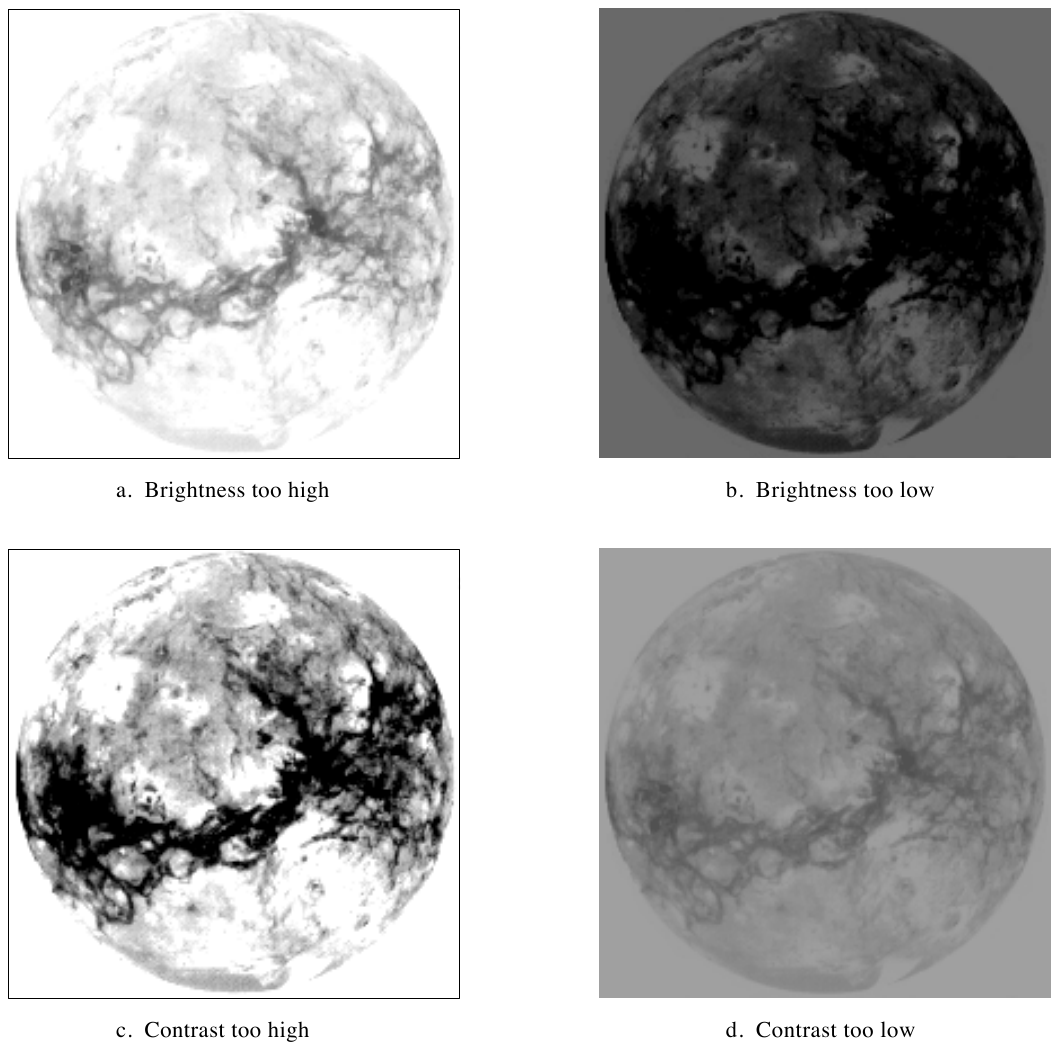
\includegraphics[width=0.883\linewidth,height=0.8\textheight,keepaspectratio]{assets/ch23/fig23-10.png}
\caption*{\textbf{图 23-10　亮度与对比度的调节。}
提高亮度会让图像中的每个像素都变亮。相比之下，提高对比度会让亮的区域更亮、暗的区域更暗。这几幅图展示了亮度和对比度调错时的效果。
（a. Brightness too high = 亮度太高；b. Brightness too low =
亮度太低；c.~Contrast too high = 对比度太高；d.~Contrast too low =
对比度太低。）}
\end{figure}

图 23-11 和 23-12 更详细地说明了亮度和对比度。图 23-12
用六种不同的亮度和对比度设置显示了一幅测试图像。图 23-11
给出了这幅测试图像的构成：一个 80×32 像素的数组，每个像素的值在 0 到 255
之间。测试图像的背景填满了在 0 到 255
之间均匀分布的随机噪声。三个方框的像素值从左到右分别为 75、150 和
225。每个方框里有两个三角形，像素值只和周围略有不同。换句话说，图像中有一块暗区带有微弱的细节，一块中等亮度的区域带有微弱的细节，还有一块亮区带有微弱的细节。

\begin{figure}[htbp]
\centering
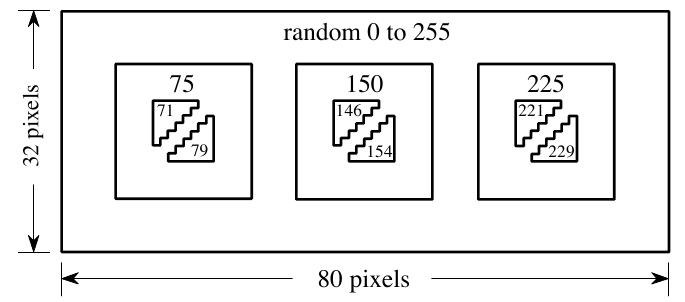
\includegraphics[width=0.571\linewidth,height=0.8\textheight,keepaspectratio]{assets/ch23/fig23-11.png}
\caption*{\textbf{图 23-11　亮度与对比度测试图像。} 这是图 23-12
所用数字图像的构成。三个方框分别构成暗、中、亮三个物体，每个里面有两个低对比度的三角形。图中标出了各区域像素的数字编号（DN）。
（random 0 to 255 = 0 到 255 的随机值，32 pixels / 80 pixels = 32 像素 /
80 像素。原书图注排在图左侧，裁图时已去掉，译文见上。）}
\end{figure}

图 23-12 展示了怎样通过调节对比度和亮度，看清图像中不同的特征。在 (a)
中，亮度和对比度设在正常水平，如图像左边的 B 和 C
滑块所示。现在请注意每幅图像旁边的曲线图，它叫输出变换(output
transform)、输出查找表(output look-up table)或伽马曲线(gamma
curve)。它控制显示图像的硬件。存储图像中每个像素的值（0 到 255
之间的一个数）经过这个查找表，得到另一个 0 到 255
之间的数。这个新的数字编号驱动视频亮度电路，0 到 255
分别对应从黑到白。也就是说，查找表把存储的数映射成显示的亮度。

图 (a)
展示了输出变换设成''什么都不做''时图像的样子，即数字输出与数字输入完全相同。噪声背景中的每个像素是一种随机的灰色，在黑白之间均匀分布。三个方框显示为暗、中、亮，彼此区分得很清楚。问题在于，每个方框里的三角形不容易看出来；对比度太低，眼睛无法把这些区域与周围区分开。

图 (b) 和 (c)
展示了改变亮度的效果。提高亮度使输出变换向左平移，降低亮度则使它向右平移。提高亮度使图像中每个像素显得更亮；反过来，降低亮度使每个像素显得更暗。这些变化可以改善图像中过暗或过亮区域的可见性，但调得太过就会使图像饱和。例如，(b)
中最右边方框里的所有像素都以满亮度显示，即 255。(c)
中则是相反的效果，最左边方框里的所有像素都显示为最黑的黑，即数字编号
0。由于这些区域中的所有像素值都相同，三角形就完全消失了。还要注意，(b)
和 (c) 中的三角形没有一个比 (a)
中更容易看到。改变亮度对于把低对比度物体从周围区分出来帮助很小（如果有的话）。

图 (d) 展示了为观察数字编号 75
附近的像素值而优化的显示。做法是调高对比度，使输出变换的斜率变大。例如，存储的像素值
71 和 75 在显示中变成 100 和 116，对比度增大了四倍。像素值 46 到 109
显示为从最黑的黑到最白的白。为增大对比度付出的代价是：像素值 0 到 45
饱和为黑，110 到 255 饱和为白。如 (d)
所示，增大对比度后可以看到左边方框里的三角形，代价是中间和右边的方框饱和了。

图 (e) 展示了把对比度进一步调高的效果，结果是在 256
个可能的存储级别中只有 16 个显示为非饱和。亮度也调低了，使这 16
个可用级别以数字编号 150
为中心。中间方框里的细节现在非常清楚，但图像中几乎所有其他部分都饱和了。例如，看看图像边框上的噪声：几乎没有中间灰色的像素，几乎每个像素不是纯黑就是纯白。这种用高对比度只看少数几个级别的技术，有时叫灰度拉伸(grayscale
stretch)。

\begin{quote}
\textbf{译注：} 原书此处写''以数字编号 175 为中心''，但图 23-12e
的标签是''DN 150 处大幅提高对比度''，曲线的陡坡也在 150
附近，而且正文接着说看清的是中间方框（像素值 150）的细节，所以应为
150，译文已改正。
\end{quote}

对比度调节是在一个较小的像素值范围上''放大''的一种方式。亮度控制则把放大的那一段对准感兴趣的像素值。大多数数字成像系统都允许按这种方式调节亮度和对比度，并且常常以图形方式显示输出变换（如图
23-12）。相比之下，电视和视频监视器上的亮度和对比度旋钮是模拟电路，工作方式可能不同。例如，监视器的对比度旋钮可能调节模拟信号的增益，而亮度旋钮可能加上或减去一个直流偏置。这里的教训是：如果这些模拟旋钮的反应和你想的不一样，不必惊讶。

\begin{figure}[htbp]
\centering
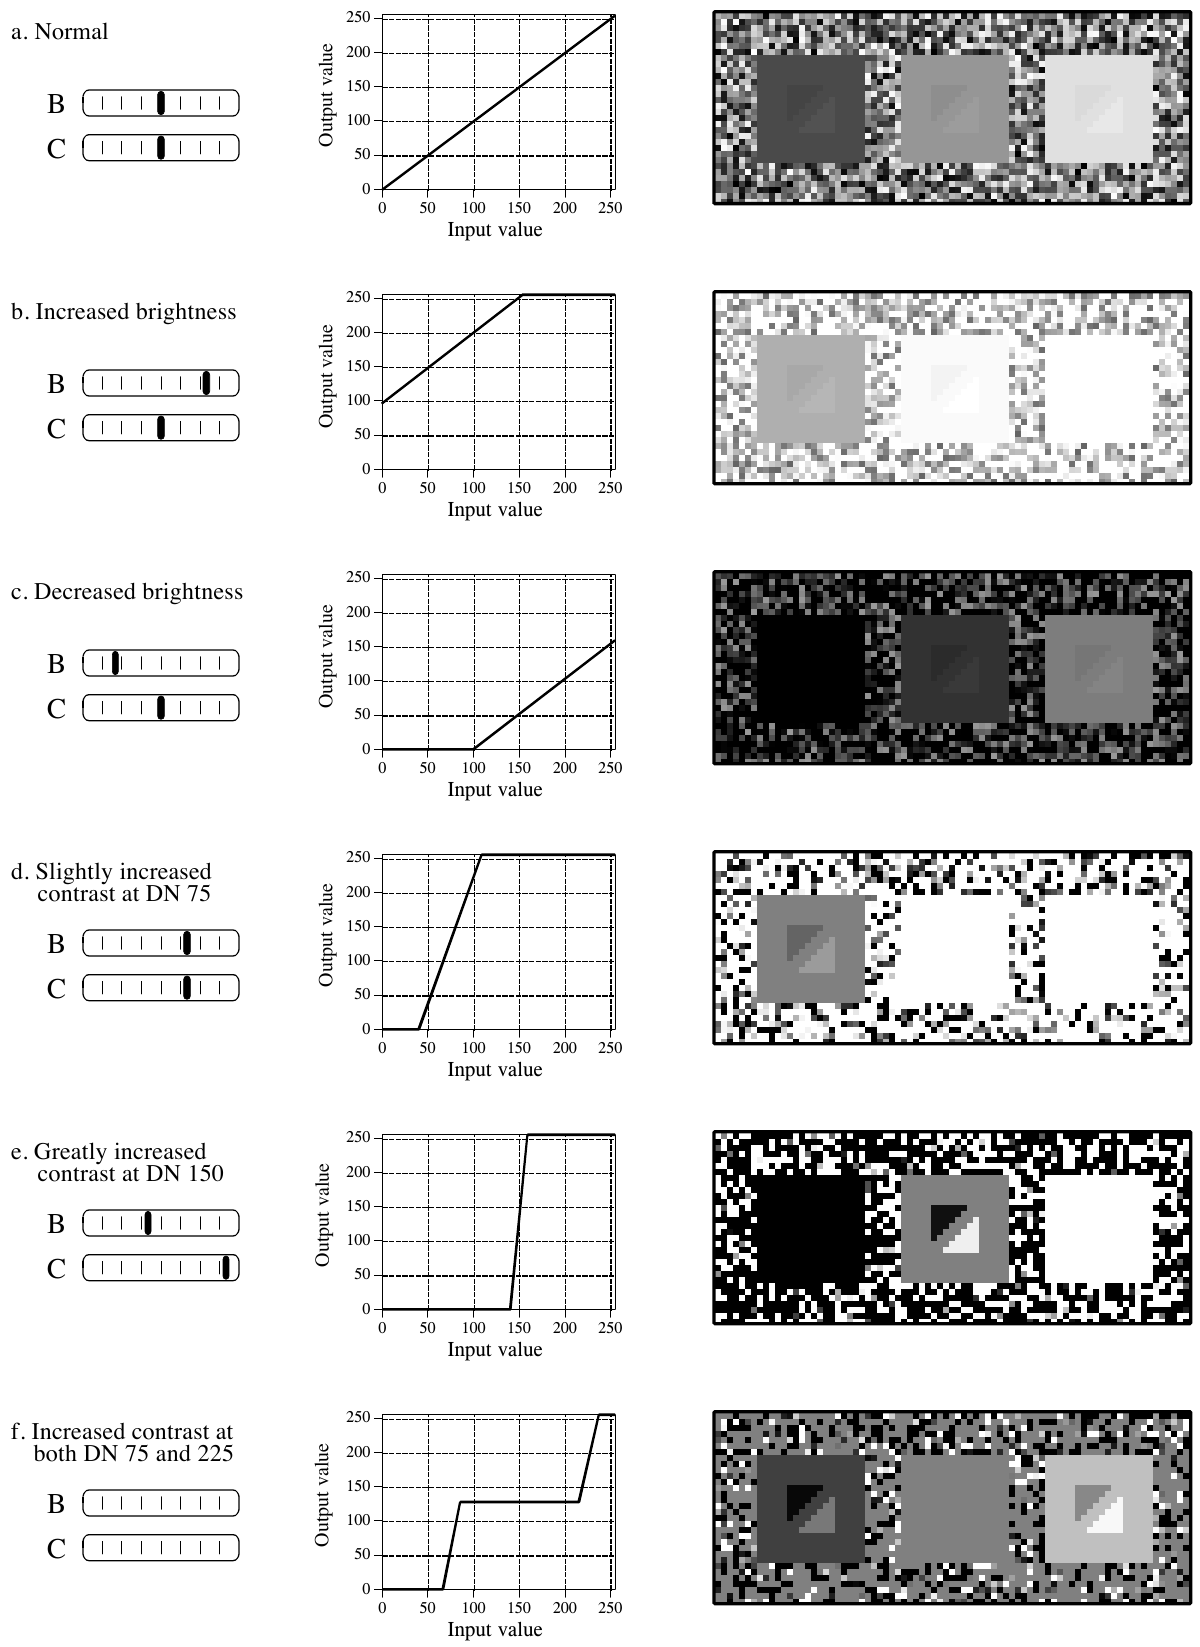
\includegraphics[width=1.000\linewidth,height=0.8\textheight,keepaspectratio]{assets/ch23/fig23-12.png}
\caption*{\textbf{图 23-12　用不同的亮度和对比度设置显示图 23-11
的测试图像。}（原书此图没有图注文字，说明见正文。）每一行左边是亮度（B）和对比度（C）滑块的位置，中间是输出变换曲线，右边是显示效果。
（a. Normal = 正常；b. Increased brightness = 提高亮度；c.~Decreased
brightness = 降低亮度；d.~Slightly increased contrast at DN 75 = 在 DN
75 处稍微提高对比度；e. Greatly increased contrast at DN 150 = 在 DN 150
处大幅提高对比度；f.~Increased contrast at both DN 75 and 225 = 同时在
DN 75 和 225 处提高对比度。Input value = 输入值，Output value =
输出值。）}
\end{figure}

\section{灰度变换}

最后一幅图像，图
23-12f，与其他几幅不同。它的曲线不是在一个输入值范围上有斜率，而是在两个范围上有斜率。这使显示能同时看到左边和右边方框里的三角形。当然，这会导致不在这些数字编号附近的像素值饱和。注意
(f)
中没有画出对比度和亮度的滑块；这种显示超出了亮度和对比度调节所能提供的范围。

沿着这个思路再走一步，就得到一种改善图像观感的强大技术：灰度变换(grayscale
transform)。思路是在我们感兴趣的像素值上提高对比度，代价是牺牲我们不关心的像素值。具体做法是规定
0 到 255
每个可能像素值的相对重要性。值越重要，在显示图像中它的对比度就做得越大。下面用一个例子来说明实现这一过程的系统方法。

\begin{figure}[htbp]
\centering
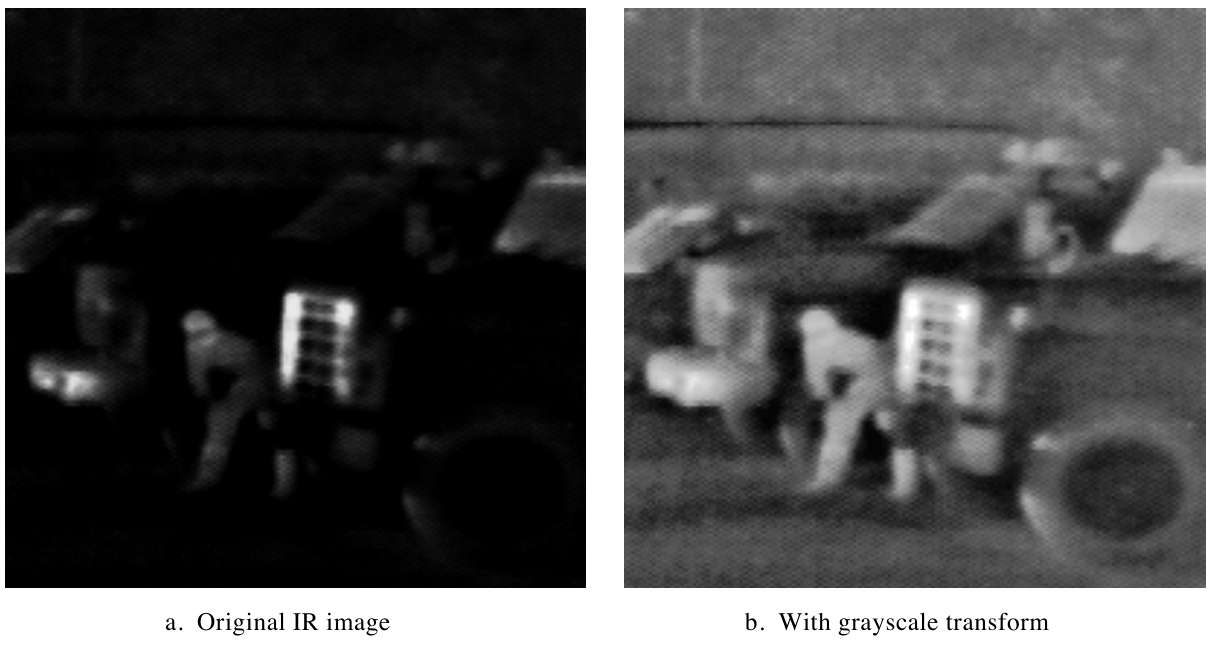
\includegraphics[width=1.000\linewidth,height=0.8\textheight,keepaspectratio]{assets/ch23/fig23-13.png}
\caption*{\textbf{图 23-13　灰度处理。} 图 (a)
是在完全黑暗中用红外相机拍摄的。图像中的亮度与温度有关，所以温暖的人体和发热的卡车格栅显得较亮。图
(b) 是用图 23-14c 所示的手工灰度变换处理后的结果。 （a. Original IR
image = 原始红外图像；b. With grayscale transform = 经灰度变换后。）}
\end{figure}

图 23-13a 中的图像，是在完全黑暗中用一台对远红外敏感的 CCD
相机拍摄的。被成像的参数是温度：物体越热，发出的红外能量越多，在图像中就越亮。这就是为什么背景很黑（冷），人体是灰色（温），卡车格栅是白色（热）。这类系统对军队和警察来说再好不过了：对方连自己都看不见的时候，你却能看见他！(a)
中的图像不好看，因为像素值分布很不均匀。图像的大部分太暗，景物中的细节看不出来。另一端，格栅已接近白色饱和。

这幅图像的直方图(histogram)如图 23-14a
所示，可以看出背景、人和格栅的像素值相当分离。在这个例子中，我们要提高背景和格栅的对比度，代价是牺牲其他一切，包括人体。图
(b) 表示了这个策略。我们规定最低的像素值（背景）的相对对比度为
12；同样，最高的像素值（格栅）的相对对比度为 6。人体的相对对比度为
1，各区域之间用阶梯过渡。所有这些值都是通过反复试验确定的。

\begin{figure}[htbp]
\centering
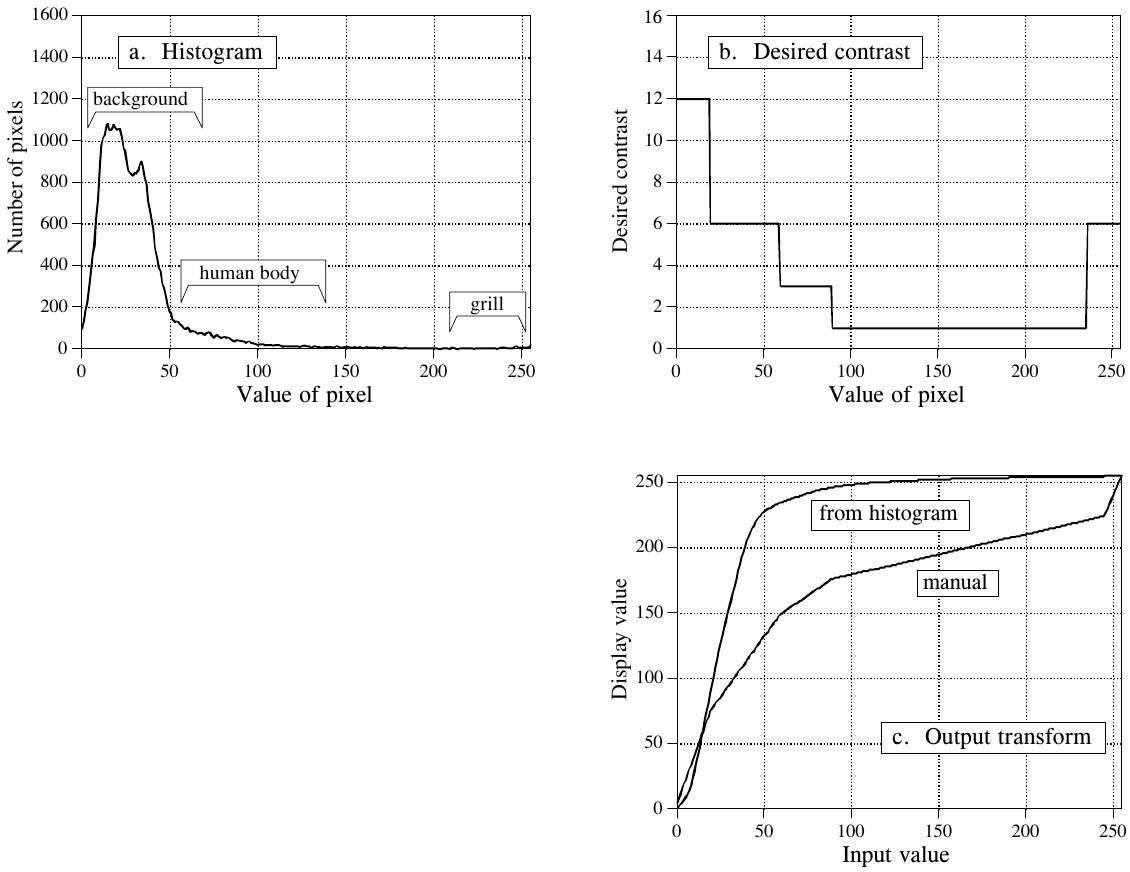
\includegraphics[width=0.942\linewidth,height=0.8\textheight,keepaspectratio]{assets/ch23/fig23-14.png}
\caption*{\textbf{图 23-14　设计灰度变换。} 图 (a) 是图 23-13a
原始图像的直方图。在 (b)
中，手工画出一条曲线，表示每个像素值所需的对比度。然后对 (b)
积分并归一化，得到输出变换的查找表（LUT），即 (c) 中标为
manual（手工）的曲线。在直方图均衡化中，则是对 (a)
中原始图像的直方图积分并归一化来得到查找表，结果也画在 (c) 中。 （a.
Histogram = 直方图，Number of pixels = 像素个数，Value of pixel =
像素值，background = 背景，human body = 人体，grill = 格栅；b. Desired
contrast = 期望的对比度；c.~Output transform = 输出变换，Display value =
显示值，Input value = 输入值，from histogram = 由直方图得到，manual =
手工。原书图注排在图左下，裁图时已去掉，译文见上。）}
\end{figure}

由这个策略得到的灰度变换如 (c) 所示，标为 manual（手工）。求法是对 (b)
中的曲线求累加和（即离散积分），再归一化，使它在最右端的值为
255。为什么要用积分来求所需的曲线？可以这样想：某个像素值处的对比度，等于输出变换在该处的斜率。也就是说，我们希望
(b) 是 (c) 的导数（斜率）。这意味着 (c) 必须是 (b) 的积分。

把图 23-13a 的图像经过这个手工确定的灰度变换，就得到图
(b)。背景变亮了，格栅变暗了，两者的对比度都更好。这些改善是以牺牲人体的对比度为代价的，入侵者的图像细节变少了（不过原图里也不能再差多少了）。

灰度变换可以显著改善图像的可观看性。问题在于，它可能需要大量的反复试验。直方图均衡化(histogram
equalization)是把这个过程自动化的一种方法。注意，(a) 中的直方图与 (b)
中的对比度加权曲线大体形状相同。直方图均衡化不加判断地直接把直方图用作对比度加权曲线，省去了人的判断。也就是说，输出变换通过对直方图（而不是手工画的曲线）积分并归一化得到。这样，像素数最多的那些值就得到最大的对比度。

直方图均衡化是一个有趣的数学过程，因为它使图像的熵(entropy)最大化，熵衡量的是固定位数能传递多少信息。直方图均衡化的毛病在于，它把某个值上像素的数量多少，误当成了该值上像素的重要程度。例如，卡车格栅和人类入侵者是图
23-13
中最显著的特征。尽管如此，直方图均衡化几乎会完全忽略这些物体，因为它们包含的像素相对很少。直方图均衡化又快又简单。只要记住：如果效果不好，手工画的曲线大概会好得多。

\section{图像变形}

拍摄行星表面的问题之一，是球面弯曲造成的变形。例如，假设你用望远镜拍摄行星中心附近的一块方形区域，如图
23-15a 所示。几个小时后，行星绕轴自转，看起来就成了 (b)
的样子。先前拍过的区域因为靠近行星的地平线而弯曲，显得严重变形。这两幅图像都包含了这个区域的完整信息，只是视角不同。拍到的是
(a) 这样的照片、但真正想要的是 (b)
那样的图像（或者反过来），这种情况相当常见。例如，一颗测绘行星表面的卫星可能从正上方拍几千张图像，就像
(a)。要做出整颗行星的自然图像（比如图 23-1
的金星图像），每幅图像都必须变形并放到正确的位置。另一方面，考虑一颗气象卫星观察一个不在它正下方的飓风。这时别无选择，只能斜着拍，就像
(b)。然后再把图像转换成从正上方看的样子，就像 (a)。

\begin{figure}[htbp]
\centering
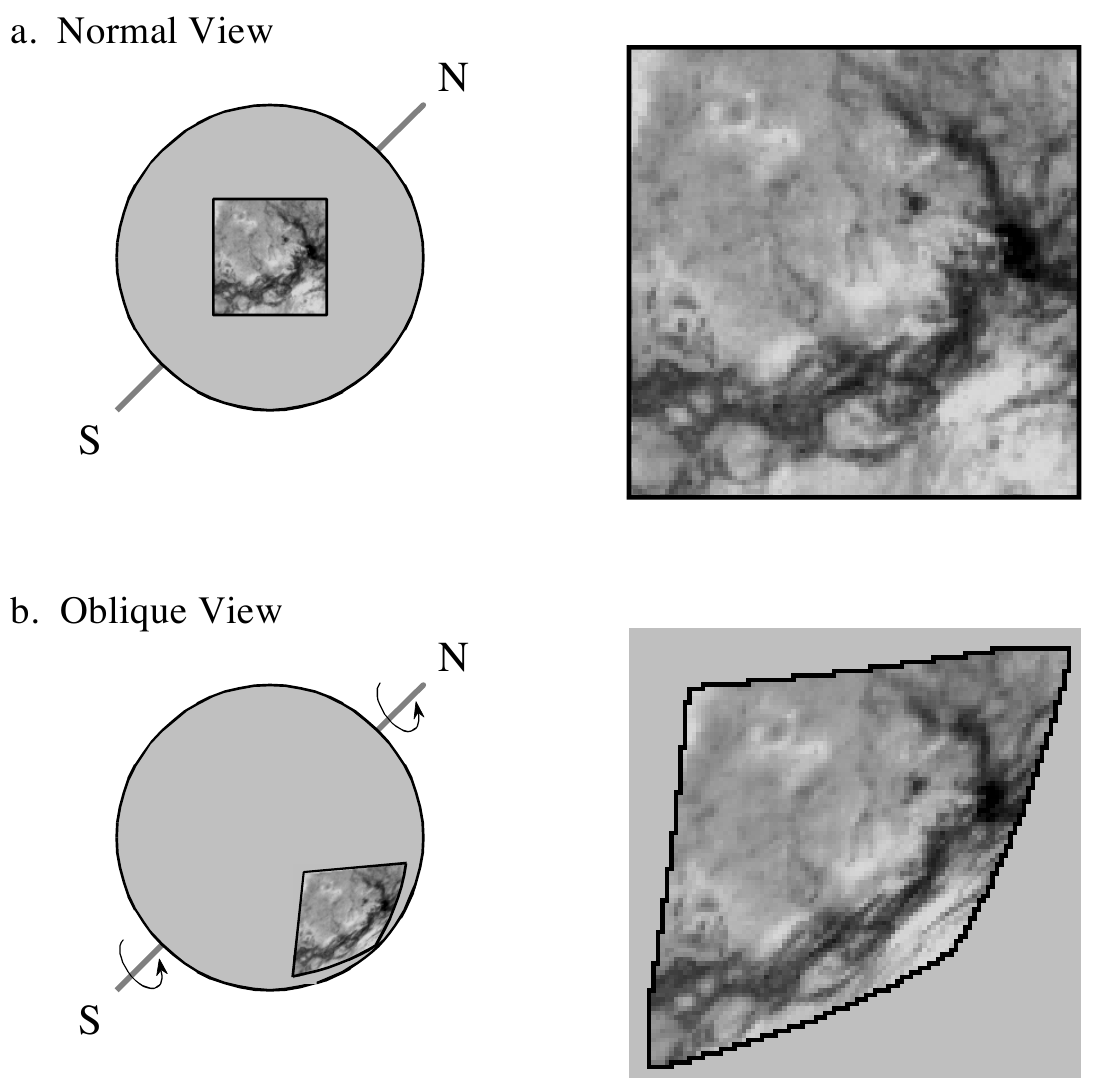
\includegraphics[width=0.912\linewidth,height=0.8\textheight,keepaspectratio]{assets/ch23/fig23-15.png}
\caption*{\textbf{图 23-15　图像变形。} 如 (a)
所示，从正面看行星上的一小块区域，几乎没有变形。相比之下，斜着看则有明显的空间变形。图像变形就是把其中一幅图像变成另一幅的技术。
（a. Normal View = 正面视图；b. Oblique View = 斜视图；N / S = 北 /
南，指行星的自转轴两极。）}
\end{figure}

这类空间变换叫做图像变形(warping)。太空摄影是图像变形最常见的用途，但还有别的用途。例如，许多真空管成像探测器都有不同程度的空间畸变，包括军用夜视相机和医用
X
光探测器。数字变形（或者你喜欢的话，叫去变形(dewarping)）可以用来校正这些器件固有的畸变。电影特效师非常喜欢对图像做变形。例如，一种叫变形动画(morphing)的技术，在一系列帧中逐渐把一个物体变成另一个。这可以造出诸如孩子变成大人、男人变成狼人之类的幻象。

图像变形接收原图像（一个二维数组），生成变形后的图像（另一个二维数组）。做法是遍历变形图像中的每个像素，并问：这里应该放什么像素值？给定变形图像中正在计算的行和列，原图像中就有一个对应的行和列。把原图像中的像素值转移到变形图像中，算法就完成了。按图像处理的行话，原图像中像素来自的那个行和列叫做来源地址(comes-from
address)。把每个像素从原图像转移到变形图像是容易的部分。难的部分是算出变形图像中每个像素对应的来源地址。这通常是一个纯数学问题，可能相当复杂。只在水平或垂直方向拉伸图像要容易些，只需把行号和/或列号乘一个系数就能得到来源地址。

图像变形中用到的技术之一是亚像素插值(subpixel
interpolation)。例如，假设你推导出了一组方程，能把变形图像中的行列地址转换成原图像中的来源地址。考虑要求变形图像中第
10 行、第 20 列像素的值时会发生什么。你把信息''行 = 10，列 =
20''代入方程，得出：来源行 = 20.2，来源列 =
14.5。关键在于，你的计算很可能用浮点数，因此来源地址不会是整数。最简单的方法是最近邻(nearest
neighbor)算法，即把地址四舍五入到最近的整数。这很简单，但在物体边缘可能产生很粗糙的颗粒感，那里的像素看起来会稍有错位。

双线性插值(bilinear interpolation)要多花一点力气，但图像质量明显更好。图
23-16 展示了它的做法。你知道分数地址周围四个像素的值，也就是第 20 和 21
行、第 14 和 15 列的像素值。本例中假设这些像素值为 91、210、162 和
95。问题是在这四个值之间插值。这分两步完成。第一步，在第 14 和 15
列之间沿水平方向插值，得到两个中间值：第 20 行上的 150.5 和第 21 行上的
128.5。第二步，在这两个中间值之间沿垂直方向插值，得到双线性插值后的像素值
139.5，再把它转移到变形图像中。为什么先水平插值、再垂直插值，而不是反过来？无所谓；不论用哪种顺序，最终答案都一样。

\begin{quote}
\textbf{译注：} 按文中给定的来源行 20.2，垂直方向的插值应为
\(150.5 + 0.2 \times (128.5 - 150.5) = 146.1\)，而不是 139.5。139.5
是两个中间值的平均，对应的是行 20.5。图 23-16a 也标的是 20.2 和
139.5，这处数值原书前后不一致；方法本身没有问题。
\end{quote}

\begin{figure}[htbp]
\centering
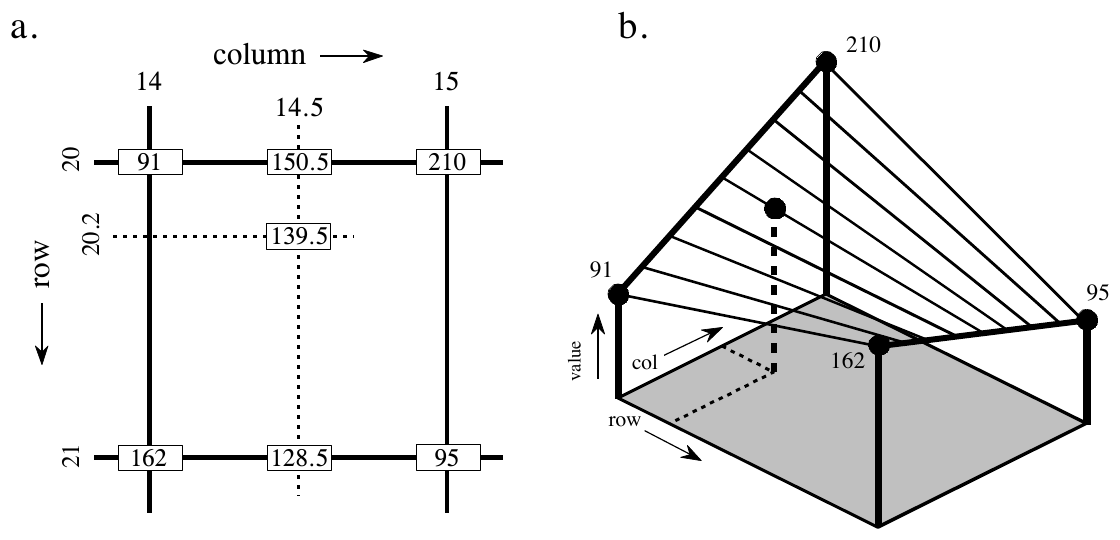
\includegraphics[width=0.933\linewidth,height=0.8\textheight,keepaspectratio]{assets/ch23/fig23-16.png}
\caption*{\textbf{图 23-16　亚像素插值。}
图像变形中的亚像素插值通常用双线性插值完成。如 (a)
所示，先沿水平方向线性插值，算出两个中间值；再在这两个中间值之间沿垂直方向线性插值，得到最终值。如
(b) 的三维示意图所示，这个过程唯一地确定了四个角上已知像素之间的所有值。
（column = 列，row = 行，value = 值，col = 列。）}
\end{figure}
